\documentclass[11pt]{article}
\usepackage[margin=1in]{geometry}
\usepackage{graphicx}
\usepackage{booktabs}
\usepackage{amsmath}
\usepackage[hidelinks]{hyperref}
\usepackage{xcolor}

\title{Placement Beats Budget:\\Four Measured Laws of Low-Bit LLM Inference on Commodity Hardware}
\author{Federico Sciuca\\\small Independent researcher \quad \texttt{federicosciuca@gmail.com}\\\small Code, raw logs, and pre-registrations: \url{https://github.com/FedericoTs/quantprobe}}
\date{July 2026}

\begin{document}
\maketitle

\begin{abstract}
We report four empirical laws of quantized large-language-model inference, derived from months of
falsification-oriented experiments conducted on a single 2016 desktop (Intel i5-7600K, NVIDIA GTX
1060 6\,GB, 16\,GB DDR4, SATA SSD). The laws state that (1) incoherence rotation helps or destroys a
tensor depending on its effective rank (a $\sim$270{,}000$\times$ swing in perplexity damage); (2)
trained mixture-of-experts networks are informationally dense everywhere, placing a $\sim$2-bit
data-free floor on expert compression; (3) depth-wise fragility under low-bit quantization is
measurable but not predictable from architecture, requiring a 30-minute functional probe; and (4)
decode speed obeys a tiered identity, $\text{tok/s} = \eta(\text{tier}) \cdot \text{BW} /
\text{active-bytes-per-token}$, with the utilization constant $\eta$ collapsing per memory tier
across models from 7B to 744B parameters and across at least four independent inference stacks.
Our primary evidential instrument is \emph{pre-registration}: predictions were committed publicly
before measurement. Eight pre-registered predictions have been scored to date, including a
same-size control (two byte-identical 5.22\,GB GGUF files differing by 2.25 perplexity purely from
\emph{which} layers hold the protected bits), a day-zero prediction of a commercial 118B release's
published throughput within 1\%, and the subsequent execution of that same model on our 16\,GB
desktop inside a band staked before the weights were downloaded (0.2--0.4 tok/s staked; 0.38 $\pm$
0.17 measured). One near-miss is reported with the same prominence and yielded a refinement (a
context term for Law 4). All claims are reproducible from raw logs committed in-tree.
\end{abstract}

\section{Introduction}
A 2016 desktop cannot run frontier models the way a datacenter does. Rather than treating that as a
budget problem, we treat it as a placement problem: \emph{where} should every bit (quantization
precision per tensor) and every byte (memory-tier residency per weight) sit? The constraint forces
method: with one machine and no capacity for sweeps, every experiment must be chosen to
\emph{falsify} a hypothesis, and every claim must survive a held-out metric.

This paper collects what survived. The result is not a bag of tricks but four laws with an unusual
evidential profile for systems work: pre-registered predictions scored in public, a byte-identical
control experiment, third-party retrodictions on hardware we have never touched, and documented dead
ends (dynamic top-$k$ expert reduction, semantic paging, dense self-speculation) that redirect the
field's attention from plausible-but-dead levers.

\section{Methodology}
\textbf{Falsification first.} Each law below is stated with its establishing measurement and at
least one prediction that would have refuted it. Negative results are reported alongside positive.

\textbf{Pre-registration.} Numeric predictions are committed to a public git repository
\emph{before} the corresponding measurement; the commit timestamp is the proof of priority. Eight
predictions have been scored: seven hits and one near-miss (Section~\ref{sec:validation}); the
near-miss is published with equal prominence and produced Law 4's context term.

\textbf{Held-out metric.} Quality claims use WikiText-2 perplexity under fixed evaluation windows
--- a corpus none of our recipes are tuned on. In-domain benchmark scores (e.g.\ coding suites for
coding-calibrated compression) are treated as insufficient, since domain-calibrated interventions
grade themselves on their own homework.

\textbf{One box, plus the world.} All primary measurements come from one machine, stated exactly.
Generalization is tested by \emph{retrodicting published third-party numbers} --- an inference
engine in pure C streaming a 744B model \cite{colibri}, a commercial 118B release on NVIDIA GB10,
and a community 284B record on AMD Strix Halo --- from their configurations alone.

\section{The Four Laws}

\subsection{Law 1 --- Rotation is rank-conditional}
Incoherence rotations (QuIP\#/QTIP/QuaRot-family preprocessing) are widely treated as universally
beneficial. Measured on matched tensors, the same rotation costs $+0.006$ perplexity on a full-rank
MLP and $+1623$ perplexity on a low-rank KV-latent bottleneck: a $\sim$270{,}000$\times$ swing
governed by effective rank alone. \emph{Consequence:} rotate full-rank tensors only; rank-check
first. \emph{Falsifiable:} a low-rank tensor that benefits from incoherence rotation at matched bits
would refute the law.

\subsection{Law 2 --- Trained networks are dense everywhere}
In the MoE models probed, experts sit at the Gaussian rate--distortion floor (no compressible slack
at fixed bits); routing is flat across domains (prose and code activate near-identical expert sets,
Jaccard 1.00 over generation horizons); activations are diffuse; and 1-bit quantization collapses
($+253$ perplexity) under every codec tried. Two-bit is the data-free floor. \emph{Consequence:}
there is no free sparsity at inference time; capacity interventions (e.g.\ calibrated expert
pruning) are domain-specialization trades, not free compression (a pre-registered out-of-domain
test of a 50\%-pruned checkpoint is open at time of writing). \emph{Falsifiable:} a data-free 1-bit
expert quantization without collapse, or a stable ``hot'' expert subset, would refute it.

\subsection{Law 3 --- Fragility is measurable, not predictable}
\label{sec:law3}
Which layers break under low-bit quantization varies by model family in ways no weight statistic we
tested predicts: Gemma-family models break in \emph{late} layers ($\sim$4$\times$ perplexity
damage), Qwen late ($\sim$2--3$\times$), Mistral --- an architectural near-twin of Qwen ---
\emph{early} ($\sim$25$\times$). A $\sim$30-minute functional probe (quantize one depth band at a
time; measure perplexity) resolves the fragility curve exactly.

The cleanest evidence that placement, not budget, is the operative variable is a byte-identical
control (Figure~\ref{fig:placement}): two GGUF files of Gemma-4-12B, same quantizer, same type
counts, same 5.22\,GB size to the byte, differing only in \emph{which} twelve FFN blocks receive
the protected type. Protecting the first twelve layers scores 12.27 perplexity; protecting the last
twelve scores 10.02. Uniform 2-bit scores 14.41. Placement alone is worth roughly twice the byte
budget.

\begin{figure}[t]
\centering
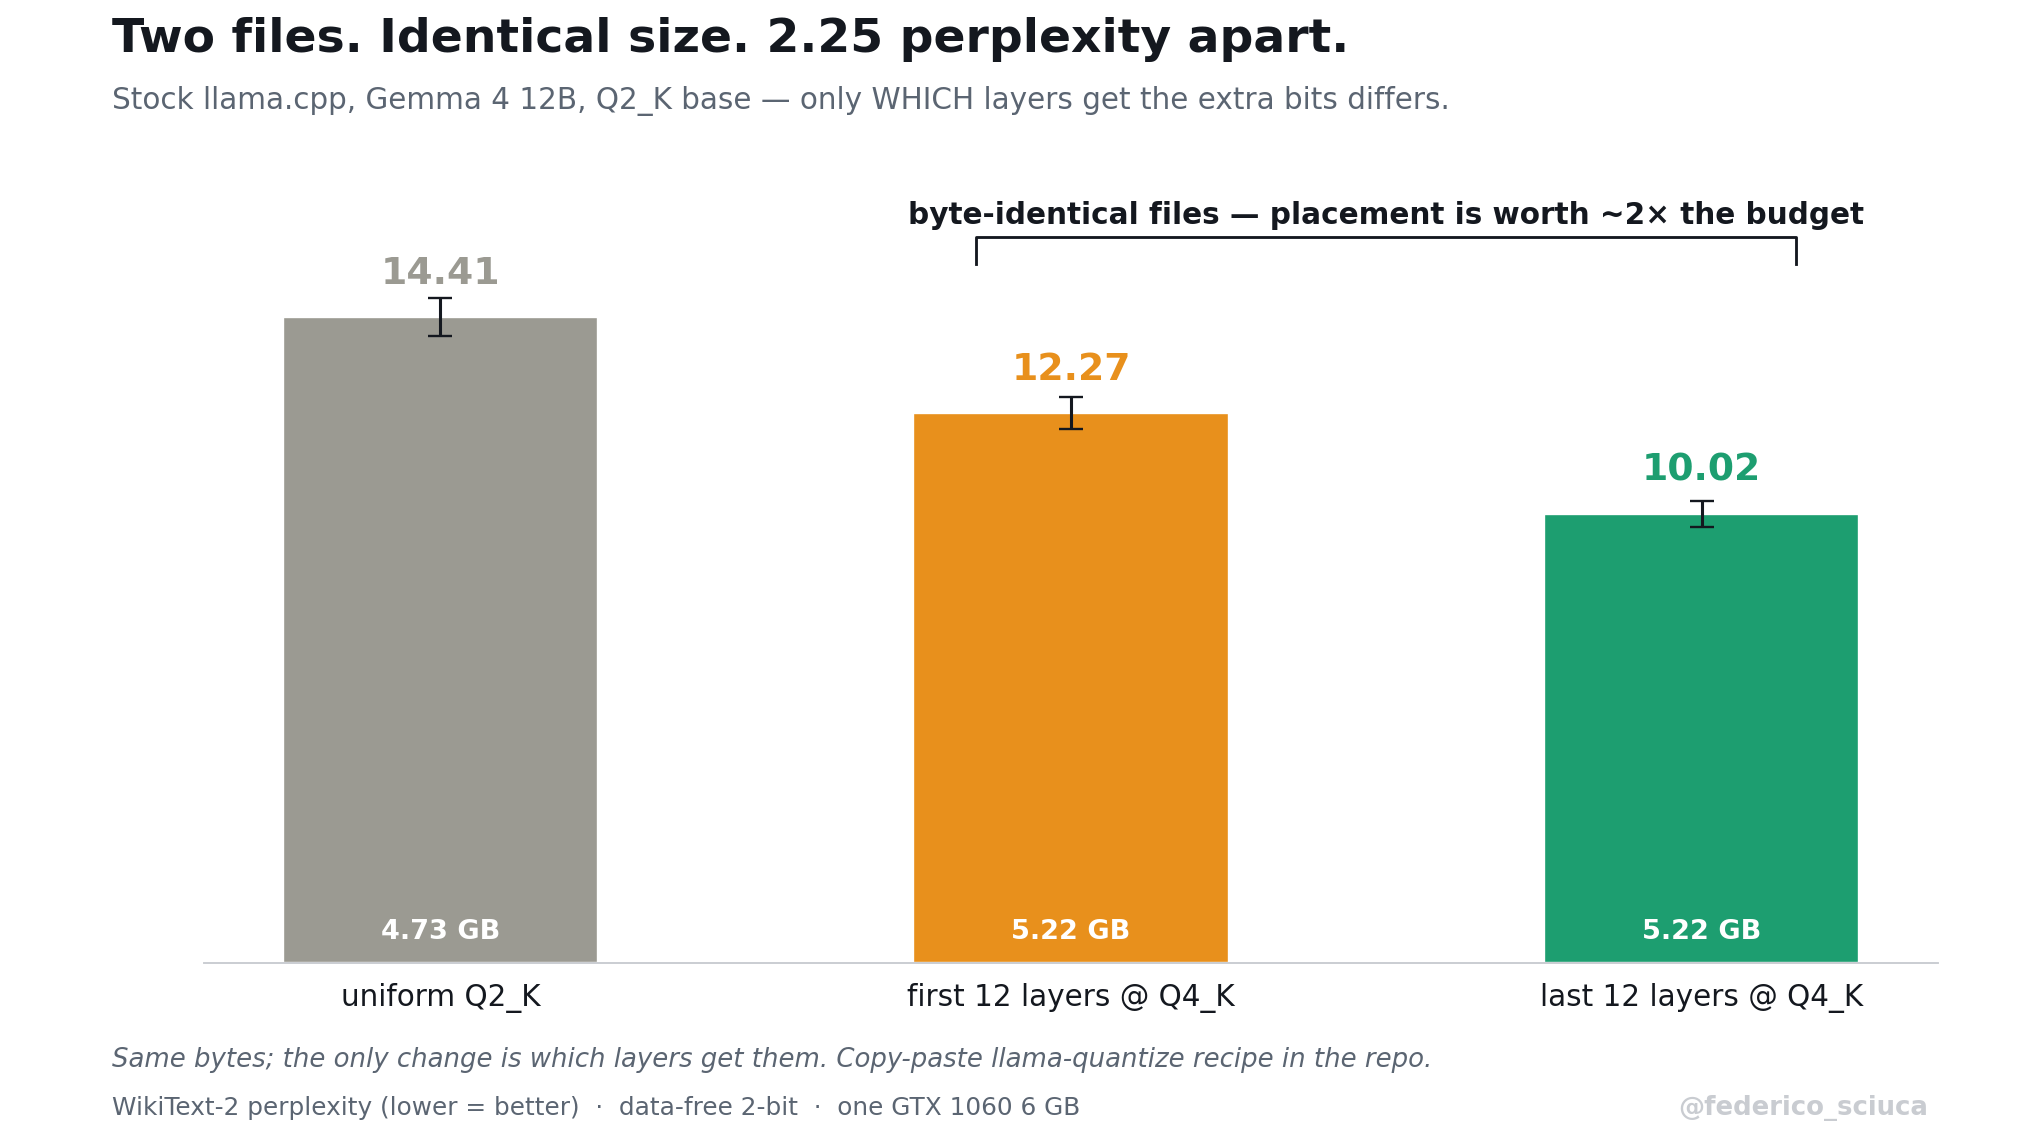
\includegraphics[width=0.9\linewidth]{x_chart_D_placement.png}
\caption{Byte-identical files, 2.25 perplexity apart. The only difference is which layers hold the
protected bits.}
\label{fig:placement}
\end{figure}

\begin{figure}[t]
\centering
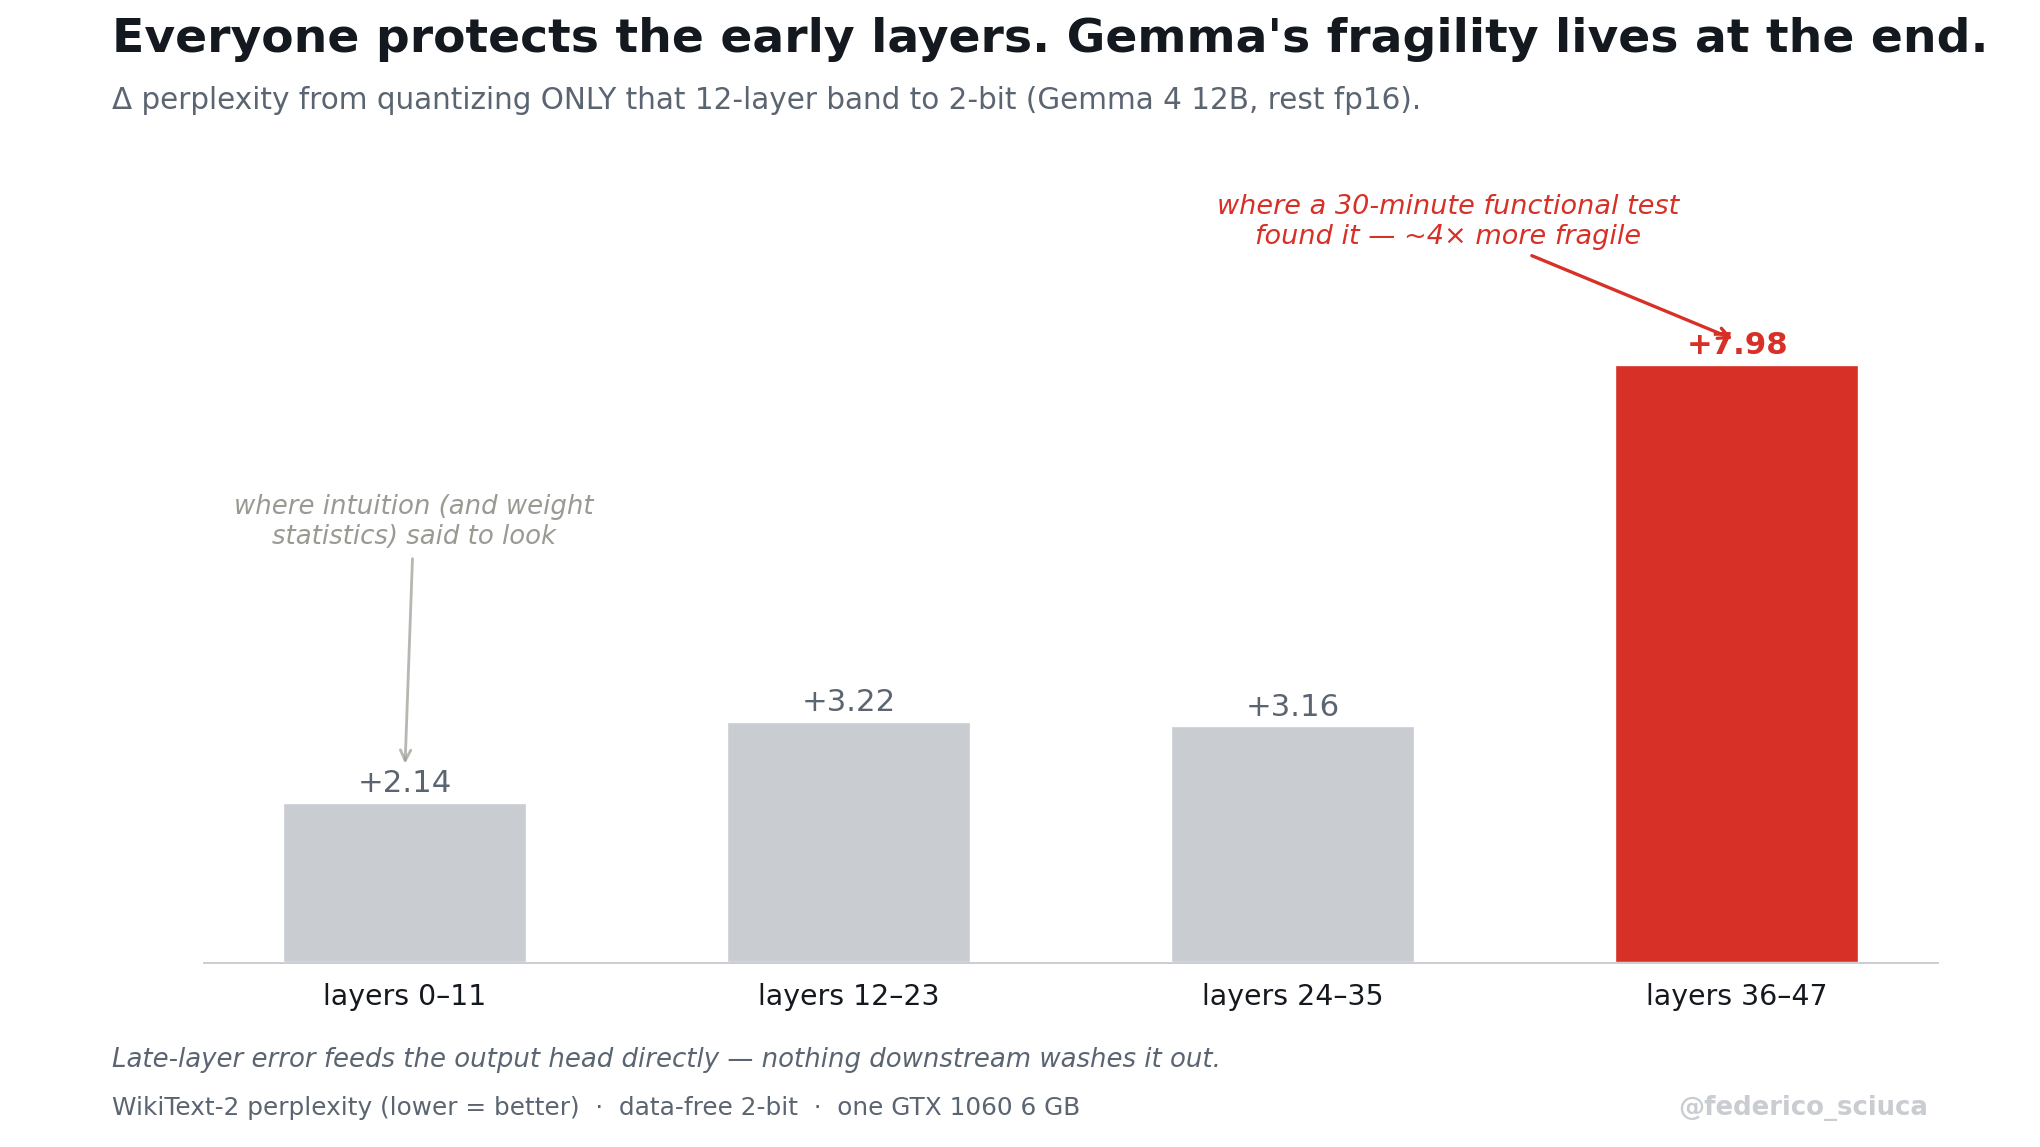
\includegraphics[width=0.9\linewidth]{x_chart_C_depthcurve.png}
\caption{Depth-fragility curve from the 30-minute probe: the spike is the fragile band; the
depth-aware recipe follows mechanically.}
\label{fig:curve}
\end{figure}

\subsection{Law 4 --- The tiered decode law}
Single-stream decode speed is a placement identity:
\begin{equation}
\text{tok/s} \;=\; \frac{\eta(\text{tier}) \cdot \text{BW}_{\text{tier}}}{\text{active-bytes-per-token}},
\end{equation}
with $\eta$ collapsing per memory tier: $\approx 0.56$ (VRAM, mid-bit), $0.29$--$0.68$ (system RAM;
dense $\approx 0.65$, MoE $\approx 0.35$ --- the expert-scatter penalty), $0.88$--$1.0$ (single-disk
streaming). On weak GPUs, low-bit decode utilization collapses ($\eta \to 0.04$ measured on Pascal
at 2-bit), making expert offload to CPU a $+54\%$ one-flag win. Speculative decoding is antagonistic
to MoE sparsity on bandwidth-bound tiers: verify batches union $\sim$40 experts versus 8, measured
2.3$\times$ \emph{slower} with a draft; a commercial release's published load-decay curve
(76.7$\to$47.5$\to$34.9$\to$24.5 tok/s at 1--8$\times$ load) matches this mechanism, and its
single-stream figure back-solves to $\eta = 1.29$ --- impossible in one memory pass, revealing
speculation from throughput arithmetic alone.

\textbf{v2: the context term.} A community reviewer correctly observed the identity above is a
short-context law: each generated token also re-reads the entire KV cache from \emph{whichever tier
KV resides on}. Measured on our box (warm-up-controlled): 20.02 $\pm$ 0.02 tok/s at depth 0 versus
16.12 $\pm$ 0.06 at depth 16{,}384 ($-19.5\%$, against a pre-registered $-8$ to $-15\%$: a
near-miss whose residual is depth-dependent attention compute on Pascal-class hardware). The term
recurses the law: KV placement matters exactly as weight placement does, and KV also consumes
capacity on its tier --- large contexts can flip the optimal placement or evict feasibility
(Figure~\ref{fig:kv}).

\begin{figure}[t]
\centering
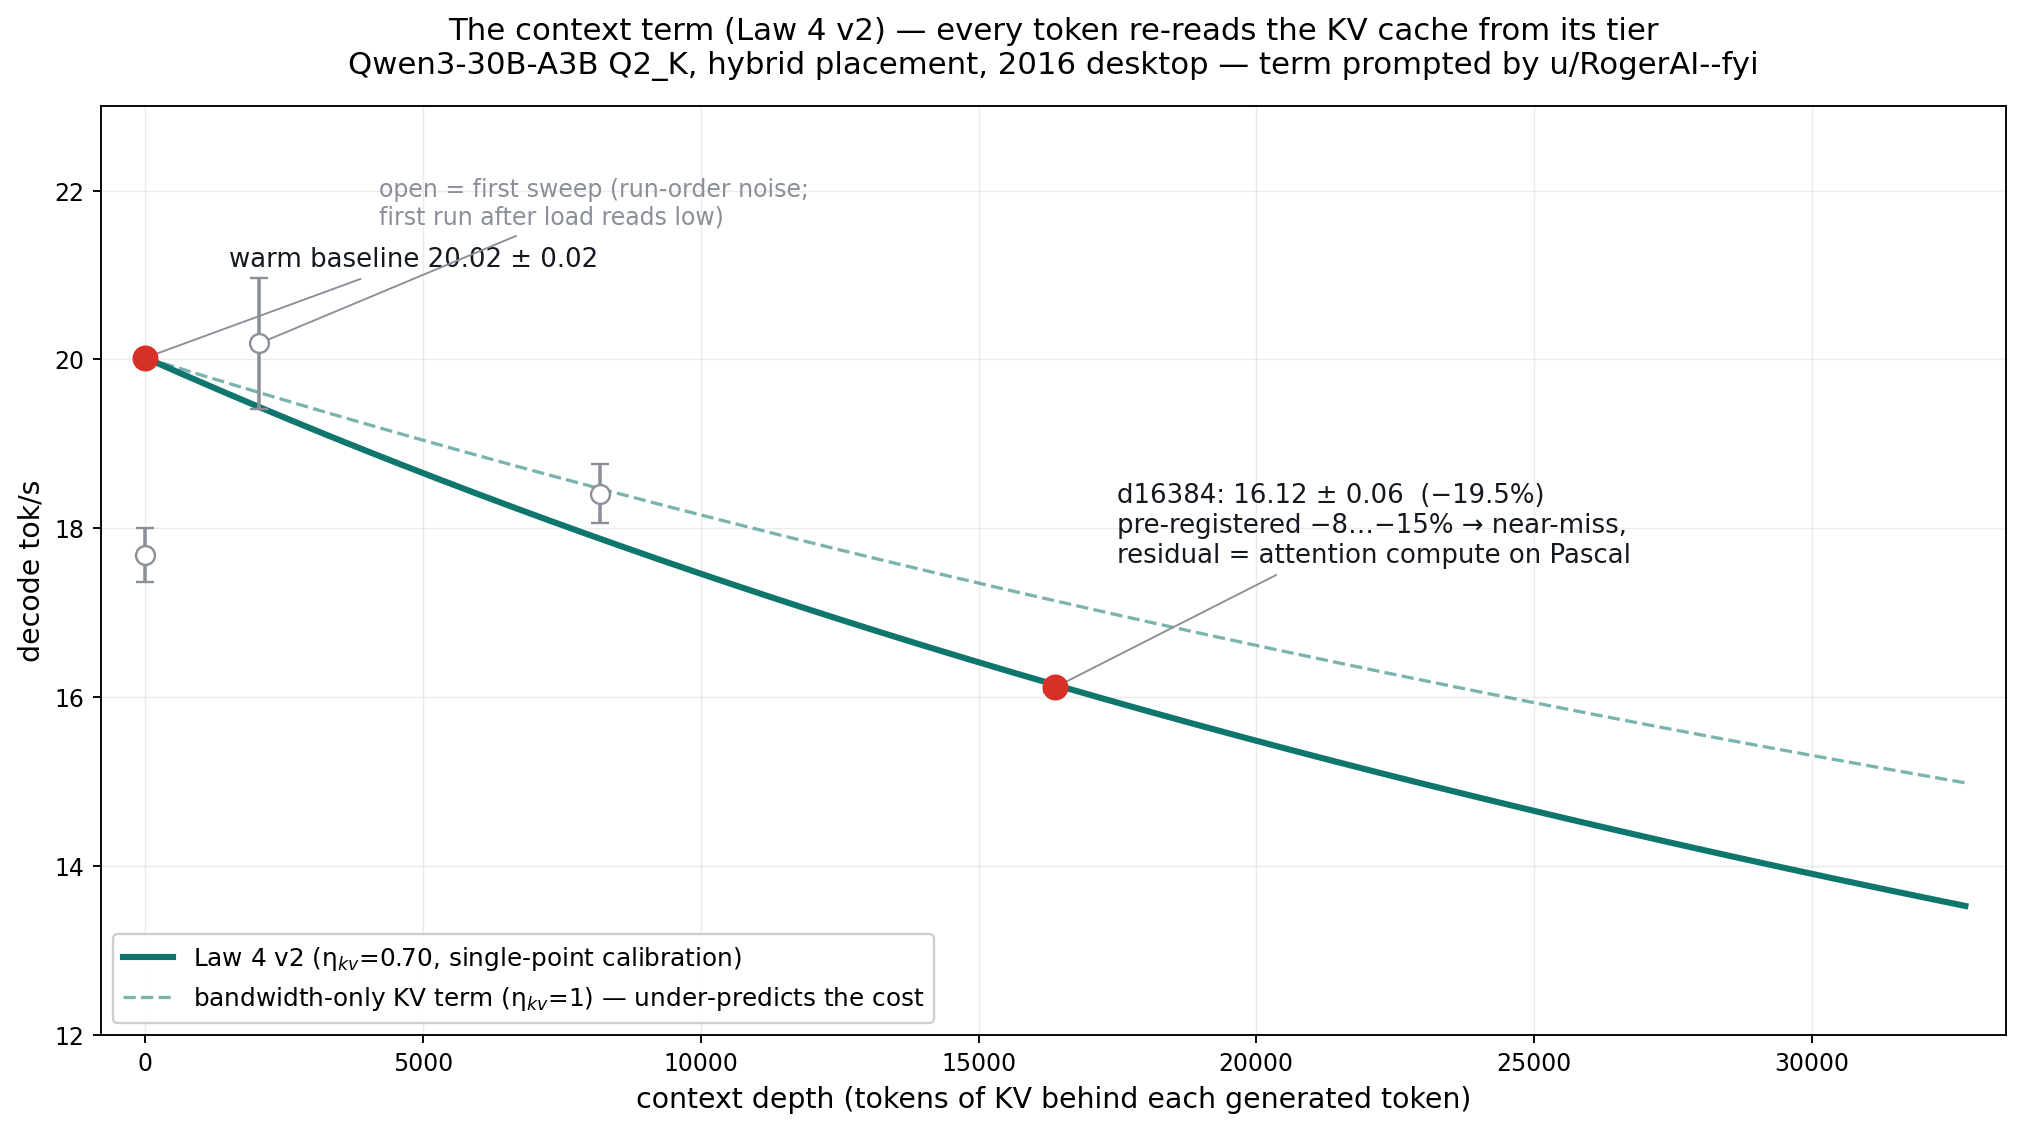
\includegraphics[width=0.9\linewidth]{x_chart_I_kvdepth.png}
\caption{The context term: decode versus KV depth, measured against the law
($\eta_{kv} = 0.70$, single-point calibration; pre-registered band and near-miss annotated).}
\label{fig:kv}
\end{figure}

\section{Pre-registered validation}
\label{sec:validation}
Table~\ref{tab:prereg} lists every scored prediction. Each was committed publicly before
measurement; raw logs are in-tree.

\begin{table}[t]
\centering
\small
\begin{tabular}{lll}
\toprule
Prediction (committed first) & Measured (after) & Verdict \\
\midrule
110B (GLM-4.5-Air) streamed from SATA: 0.2--0.3 tok/s & 0.19 & hit \\
RAM overclock (2133$\to$3000) scales dense decode $\times$1.41+ & $\times$1.52 & hit \\
30B MoE hybrid placement: $\sim$19 tok/s & 19.30 $\pm$ 0.88 & hit \\
Laguna S 2.1 (118B) on DGX Spark, from config alone: $\sim$47 & 47.5 (published) & hit ($<$1\%) \\
Laguna S 2.1 on \emph{this} desktop, staked pre-download: 0.2--0.4 & 0.38 $\pm$ 0.17 & hit \\
KV-depth 16k: $-8$ to $-15\%$ & $-19.5\%$ & near-miss \\
colibri's published 744B tiers, from our $\eta$ bands & inside bands & retrodiction \\
Strix Halo 284B record: leaderboard $\eta$ decomposition & 0.58/0.43/0.35 & retrodiction \\
\bottomrule
\end{tabular}
\caption{Scored pre-registrations and retrodictions. Open at time of writing: five falsifiable
predictions on a third-party engine's v1.1 features, a CPU-only context-slope band, and an
out-of-domain expert-pruning test.}
\label{tab:prereg}
\end{table}

\begin{figure}[t]
\centering
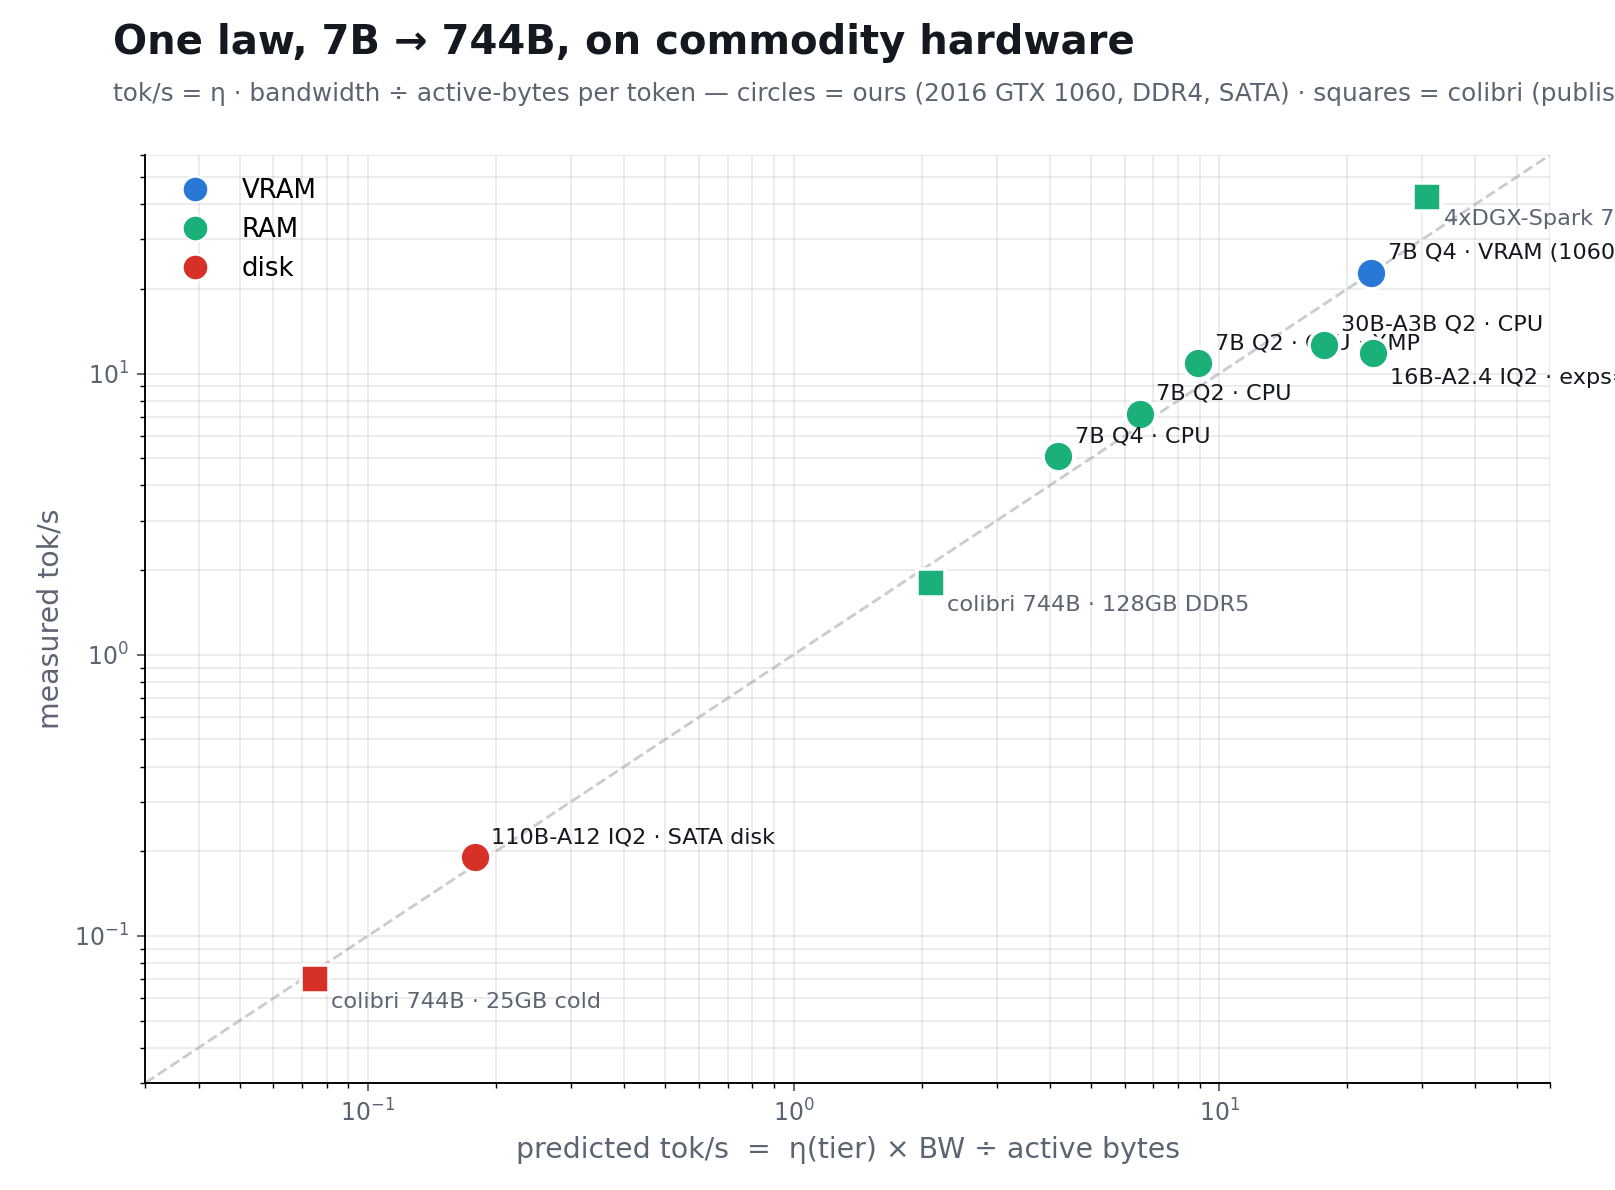
\includegraphics[width=0.9\linewidth]{x_chart_E_scalinglaw.png}
\caption{One law, 7B to 744B: predicted versus measured across our box, published third-party tiers,
and two commercial releases.}
\label{fig:law}
\end{figure}

\section{The recipe and the tool}
The laws compose into a mechanical recipe: probe the fragility curve (Law 3), protect the fragile
band and attention at $\sim$4-bit with everything else at $\sim$2-bit (Laws 2--3), place tensors by
tier bandwidth (Law 4), skip incoherence rotation on low-rank tensors (Law 1). The reference
implementation, \texttt{quantprobe} (MIT), packages this as nine commands over stock
\texttt{llama.cpp}, including hardware auto-detection, GGUF-derived model specification, and an
opt-in (fully user-reviewed, zero-telemetry) community loop that plots contributed
predicted-versus-measured points against the law.

\section{Convergent evidence}
Independent systems converge on the same physics: a pure-C engine streaming a 744B MoE from disk
\cite{colibri}; a commercial 118B released with 4-bit weights and speculative decoding on unified
memory; a community 284B record on AMD Strix Halo built on mixed 2/3/4-bit expert formats with
importance-matrix calibration; and calibrated expert pruning marketed as free compression, whose
value the law reprices as memory-tier promotion (capacity, not per-token speed). Each is an
instance of placement beating budget; each published number we have tested lands on the equation.

\section{Limitations}
Primary measurements come from one machine; $\eta$ values for unmeasured hardware classes ship as
falsifiable estimates, clearly tagged. WikiText-2 perplexity is our only quality metric ---
downstream-task validation is future work. The fragility atlas covers four model families: enough
to disprove universality, not to chart it. $\eta_{kv}$ and multi-device aggregation efficiencies are
single-point calibrations, offered for community falsification through the tool's measurement loop.

\section{Reproducibility}
Every number in this paper traces to a raw log committed in the public repository, following a
claim $\to$ script $\to$ log manifest. Pre-registration documents, their staking commits, the
probe/recipe tooling, the browser calculator, and all charts are in-tree at
\url{https://github.com/FedericoTs/quantprobe}.

\begin{thebibliography}{9}
\bibitem{colibri} JustVugg. \emph{colibri: run GLM-5.2 (744B MoE) on a 25GB-RAM consumer machine}.
\url{https://github.com/JustVugg/colibri}, 2026.
\bibitem{quip} Chee et al. \emph{QuIP\#: Even better LLM quantization with Hadamard incoherence}.
2024. \bibitem{gguf} Gerganov et al. \emph{llama.cpp}. \url{https://github.com/ggml-org/llama.cpp}.
\end{thebibliography}

\end{document}
